%\begin{enumerate}[label=\thesection.\arabic*.,ref=\thesection.\theenumi]
%\numberwithin{equation}{enumi}
\item For a unity feedback system 
\begin{align}
G(s) = \frac{K}{(s)(s+2)(s+4)(s+6)}
\label{eq:ee18btech11046_system}
\end{align}
Design a lag compensator to yield a $K_{v}=2$ and Phase Margin of $30\degree$
%
\solution Fig.\ref{fig:ee18btech11046_flow} models the equivalent of compensated closed loop system. 
 \begin{figure}[!ht]
	\begin{center}
		\resizebox{\columnwidth}{!}{\begin{enumerate}[label=\thesubsection.\arabic*.,ref=\thesubsection.\theenumi]
\numberwithin{equation}{enumi}
\item A feedback control system has the characteristic equation 
\begin{align}
    s^2 + 6Ks + 2s + 5 = 0, \quad K > 0. 
\label{eq:ee18btech11046_char}
\end{align}
%
Find the open loop gain.
\\
\solution     \label{eq:ee18btech11046_char} can be expressed as

\begin{align}
    1+\frac{6 k s}{s^{2}+2 s+5}&=0    
\\
\implies 1+KG(s)&=0
\\
\implies G(s) &= \frac{6 s}{s^{2}+2 s+5}
\label{eq:ee18btech11046_gs}
\end{align}

\item Find the poles and zeros of $G(s)$
\\
\solution The poles and zeros  are at 
\begin{align}
\begin{split}
p_1,p_2 &= -1 \pm 2\j
\\
z &=0
\end{split}
\label{eq:ee18btech11046_pz}
\end{align}

\item Find the number of root locus branches.
\\
\solution  For $G(s)$, let 
\begin{itemize}
\item $P$- No. of finite poles
\item $Z$- No. of finite zeros
\end{itemize}
%
The number of root locus branches
\begin{align}
N = 
\begin{cases}
P & P > Z,
\\
Z & P < Z.
\end{cases}
\end{align}
The root locus branches start at the open loop poles and end at open loop zeros. 
From \eqref{eq:ee18btech11046_pz}, 
\begin{align}
P=2, Z = 1 \implies N = 2
\end{align}
%
One branch originates at each pole and ends at zero and the other branch starts from other pole and goes to infinity.
\item Find the centroid and the angle of asymptotes.
\\
\solution 
Some of the root locus branches approach infinity when $P \ne Z$. Asymptotes give the direction of these root locus branches. The intersection point of asymptotes on the real axis is known as centroid.  The ordinate of the centroid is given by 
\begin{align}
\frac{\sum_{i=1}^{P} p_{i}-\sum_{j=1}^{Z} z_{j}}{P-Z} 
&= \frac{-2-0}{2-1}
\\
&= -2
\end{align}
%
after substituting from \eqref{eq:ee18btech11046_pz}.  Thus, the centroid is at $\brak{-2,0}$.
The formula for angle of asymptotes $\theta$ is
\begin{align}
\theta&=\frac{(2 q+1) \pi}{P-Z}, \quad q =0, 1, \dots P-Z-1
\\
&=\pi
\end{align}
%
One branch meets the real axis at a breakaway point then goes to zero at origin and other goes to infinity following the asymptote($y=0$).
	\item Find the intersection points of root locus branches with the imaginary axis. 
\\
\solution Using the Routh array method, 

\item Find the angle of departure with respect to the  pole $p_k$.
\\
\solution The angle of departure with respect to the $k$th (complex) pole is defined as 
\begin{align}
\phi_{k}^{d}&=
\begin{cases}
\pi-\phi_k, &  \text{Im}\brak{p_k} \ne 0
\\
0 & \text{Im}\brak{p_k} = 0
\end{cases}
\end{align}
where,
\begin{align}
\phi_k&=\sum_{i=1}^{P} \phase{p_i-p_k}-\sum_{j}^{Z} \phase{p_k - z_{j}}
\end{align}
%
For $p_1 = -1+2\j$, 
\begin{align}
\phi_{1} &= \phase{-1+2\j-\brak{-1-2\j}} - \phase{-1+2i-0}
\\
\implies  &= \frac{\pi}{2} + \brak{\pi - \tan^{-1}2} = \frac{3\pi}{2} - \tan^{-1}2
\end{align}
%
\item Find the angle of arrival with respect to the zero $z_k$
\\
\solution The angle of arrival with respect to the $k$th (complex) zero is defined as 
\begin{align}
\phi_{k}^{a}&=
\begin{cases}
\pi-\phi_k, &  \text{Im}\brak{z_k} \ne 0
\\
0 & \text{Im}\brak{z_k} = 0
\end{cases}
\end{align}
where,
\begin{align}
\phi_k&=\sum_{i=1}^{P} \phase{z_k-p_i}-\sum_{j}^{Z} \phase{z_k - z_{j}}
\end{align}
%
Since there are no complex zeros there is no angle of arrival.

\item Find the breakaway point for the root locus.
\\
\solution From \eqref{eq:ee18btech11046_char} and 
\eqref{eq:ee18btech11046_gs},
    \begin{align}
        K&=\frac{-\left(s^{2}+2 s+5\right)}{6 s},
\\
        \frac{d K}{d s}&=0 \implies \sbrak{1-\frac{5}{s^{2}}}=0 
\\
  \implies        s&=-\sqrt{5}
    \end{align}
%
which is the  breakaway point that lies only in the left half plane. Some information on the breakaway point is available below.
\begin{itemize}
\item While varying $K$, the point where the Root Locus enters the real axis is called th breakaway point.
\item   It is the point on a real axis segment of the root locus between two real poles where the two real closed-loop poles meet and diverge to become complex conjugates.
\item  As the root locus is symmetric about the real axis there will be two roots at the breakaway point. 

\end{itemize}
    
\item Plot the Root Locus.
\\
\solution The following code generates the desired plot in Fig. \ref{fig:ee18btech11046}.
\begin{lstlisting}
codes/ee18btech11046.py
\end{lstlisting}    


\begin{figure}[ht!]
\centering
    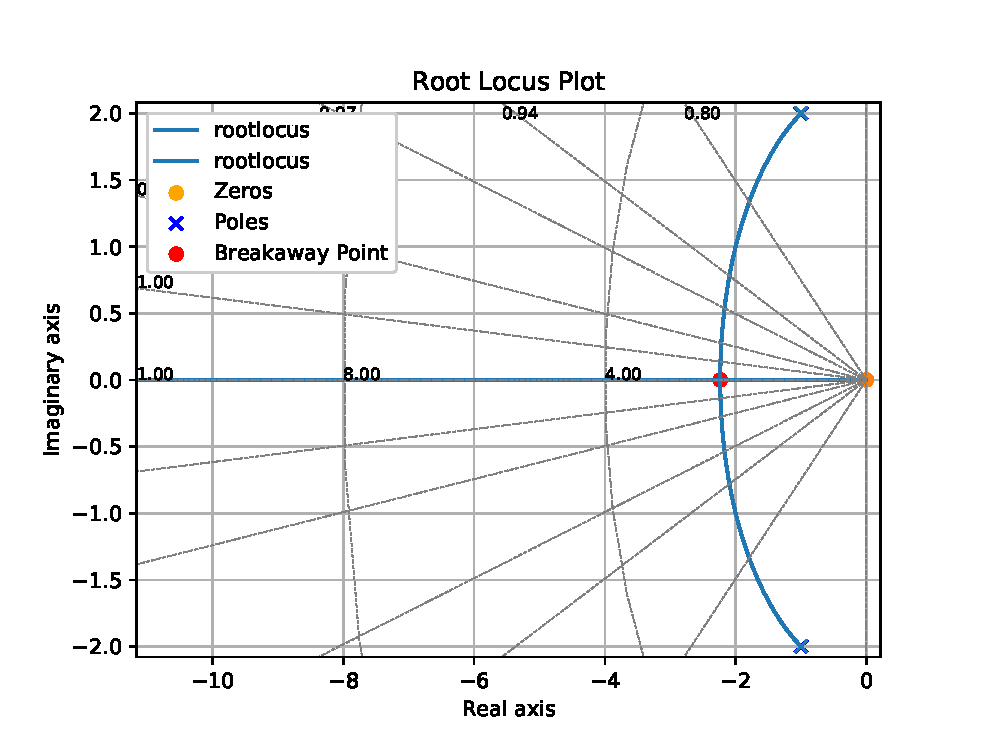
\includegraphics[width=\columnwidth]{./figs/ee18btech11046.eps}
    \caption{}
    \label{fig:ee18btech11046}
\end{figure}


\end{enumerate}

}
	\end{center}
\caption{}
\label{fig:ee18btech11046_flow}
\end{figure}

%
Static Velocity Error Constant $K_{v}$ is the steady-state error of a system for a unit-ramp input i.e.,
\begin{align}
K_{v}=\lim _{s \rightarrow 0} s G(s) G_{c}(s)
\label{eq:ee18btech11046_compansatedsys}
\end{align}
Therefore,
\begin{multline}
K_{v}=\lim _{s \rightarrow 0} s \frac{K}{s(s+2)(s+4)(s+6)} \frac{Ts+1}{\beta Ts+1}
\\
\implies 
2 = \frac{K}{(0+2)(0+4)(0+6)} \frac{T(0)+1}{\beta T(0)+1}
\\
\therefore 
K = 96
\end{multline}
\begin{align}
G\brak{s}=\frac{96}{s(s+2)(s+4)(s+6)}
\label{eq:ee18btech11046_upsys}
\end{align}


%\item The Magnitude and Phase response of G(s).\\
%\solution 
Substituting $s = \j\omega$ in \eqref{eq:ee18btech11046_upsys},
\begin{multline}
G\brak{\j\omega} =\frac{96}{\brak{j\omega}\brak{j\omega+2}\brak{j\omega+4}\brak{j\omega+6}} 
\end{multline}
\begin{multline}
\abs{G\brak{\j\omega}} = \frac{\abs{96}}{\omega\sqrt{4+\omega^2}\sqrt{16+\omega^2}\sqrt{36+\omega^2}}
\label{eq:ee18btech11046_gain}
\end{multline}
\begin{multline}
\angle G\brak{\j\omega} = -90\degree -\tan^{-1}\brak{\frac{\omega}{2}}  - \tan^{-1}\brak{\frac{\omega}{4}} \\-  \tan^{-1}\brak{\frac{\omega}{6}} 
\label{eq:ee18btech11046_phase}
\end{multline}

%\item 
The standard Transfer equation of Lag Compensator and its Phase and Gain
%\solution
\begin{align}
G_{c}\brak{s} = \frac{Ts+1}{\beta Ts+1}
\label{eq:ee18btech11046_comp}
\\
\abs{G_{c}\brak{s}} = \frac{1}{\beta}\frac{1+\brak{\frac{\omega}{T}}^{2}}{1+\brak{\frac{\omega}{\beta T}}^{2}}
\label{eq:ee18btech11046_compGain}
\\
\angle G_{c}\brak{s} = \tan^{-1}\brak{\omega T}-\tan^{-1}\brak{\omega \beta T}
\label{eq:ee18btech11046_compPhase}
\end{align}
Where $\beta > 1$.

It can be approximated that for $\omega > \frac{1}{T}$  
\begin{align}
\abs{G_{c}\brak{s}} = \frac{1}{\beta}
\label{eq:ee18btech11046_compGainapprox}
\end{align}
and Phase to be very small($<12\degree$).


%\item 
The Phase Margin(PM) of the Transfer function G(s)\\
%\solution
From \eqref{eq:ee18btech11046_gain} and \eqref{eq:ee18btech11046_gain}

At Gain Crossover,
\begin{align}
\abs{G\brak{s}} = 1
\\
\implies
\omega_{gc} = 1.47rad/sec
\\
\implies
\angle G\brak{\j \omega_{gc}} = -160.26\degree
\end{align}
\begin{align}
PM = 180\degree + \angle G\brak{\j \omega_{gc}}
\\
\implies
PM = 19.74\degree
\end{align}
The following are the Bode plots of uncompensated system
\begin{figure}[!h]
\centering
  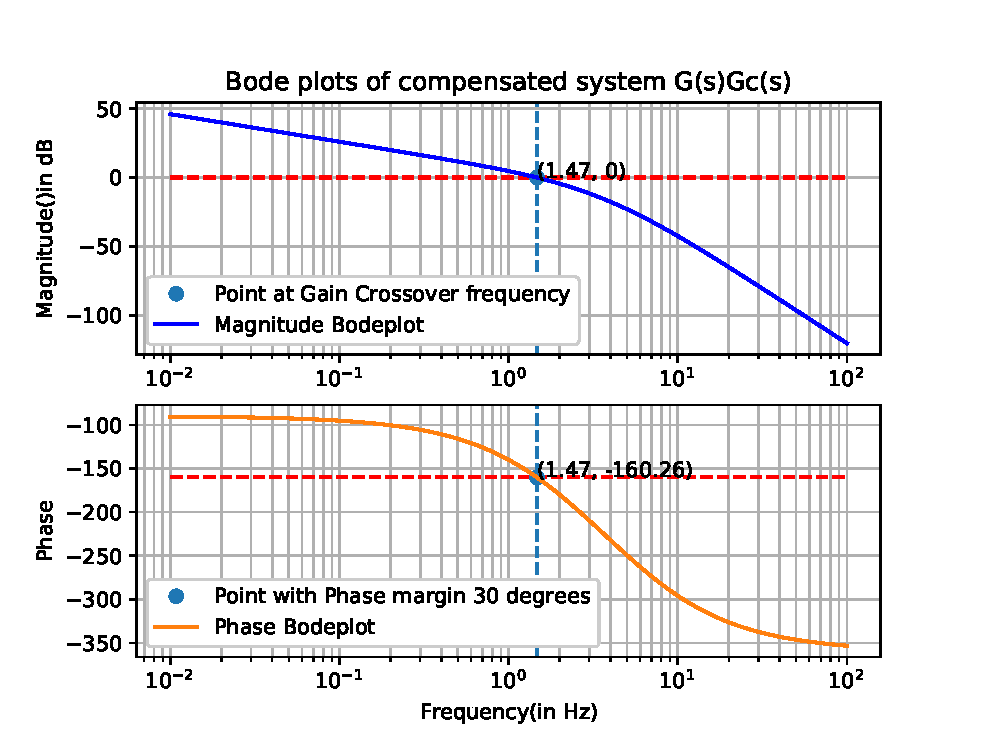
\includegraphics[width=\columnwidth]{./figs/ee18btech11046_1.eps}
\caption{}
\label{fig:ee18btech11046_uncompensated} 
\end{figure}
%

The code for Bode plots of uncompensated system 
\begin{lstlisting}
codes/ee18btech11046_1.py
\end{lstlisting}
% 



%\item Design a lag compansator such that the Phase Margin becomes $30\degree$ \\
%\solution
The lag compansator form is given in  \eqref{eq:ee18btech11046_comp},
Let
\begin{align}
G^{'}\brak{s}=G\brak{s}G_{c}\brak{s}
\end{align}
The $PM = 30\degree$ when $\angle G^{'}\brak{\j\omega} = -150\degree$ 

Since the addition of compensator reduces Gain of system, thereby reducing Gain Crossover frequency which increases Phase Margin(PM) of system.

Since, Compansator also has small negative phase(say $\epsilon$),let $\epsilon =5\degree$.i.e, $\angle G_{c}\brak{s} = 5$ 
\begin{align}
\angle G^{'}\brak{s} = \angle G\brak{s} + \angle G_{c}\brak{s}
\\
\implies
-150\degree = \angle G\brak{s} - 5\degree
\\
\implies
\angle G\brak{s} = -145\degree
\end{align}
The value of $\omega$ where $\angle G\brak{s} = -145\degree$ is 
\begin{align}
\angle G\brak{s} = -145\degree
\\
\implies
\omega_{req} = 1.10953rad/sec
\label{eq:ee18b46_omega-req}
\end{align}
The value $\frac{1}{T}$ is exactly 2 octaves below $\omega_{req}$ obtained in \eqref{eq:ee18b46_omega-req}
\begin{align}
\frac{1}{T} = \frac{\omega_{req}}{4}
\\
\implies
T = 3.605
\label{eq:ee18btech11046_T}
\end{align}
Now we should take $\beta$ such that Gain Crossover frequency occurs at $\omega_{req}$ i.e., to make $\abs{G^{'}\brak{\j\omega}} = 1$

From \eqref{eq:ee18btech11046_compGainapprox},

\begin{align}
\abs{G^{'}\brak{\j\omega_{gc}}} = \abs{G\brak{\j\omega_{gc}}}\abs{G_{c}\brak{\j\omega_{gc}}} = 1
\\
\implies
1.4936 \times \frac{1}{\beta} = 1
\\
\implies
\beta = 1.4936
\label{eq:ee18btech11046_beta}
\end{align} 
Substituting values of T and $\beta$ obtained from\eqref{eq:ee18btech11046_T} and\eqref{eq:ee18btech11046_beta} in \eqref{eq:ee18btech11046_comp}
The required Compensator Transfer is
\begin{align}
G_{c}\brak{s} = \frac{3.605s+1}{5.384s+1}
\end{align}
The following are the Bode plots of compensated system
\begin{figure}[!h]
\centering
  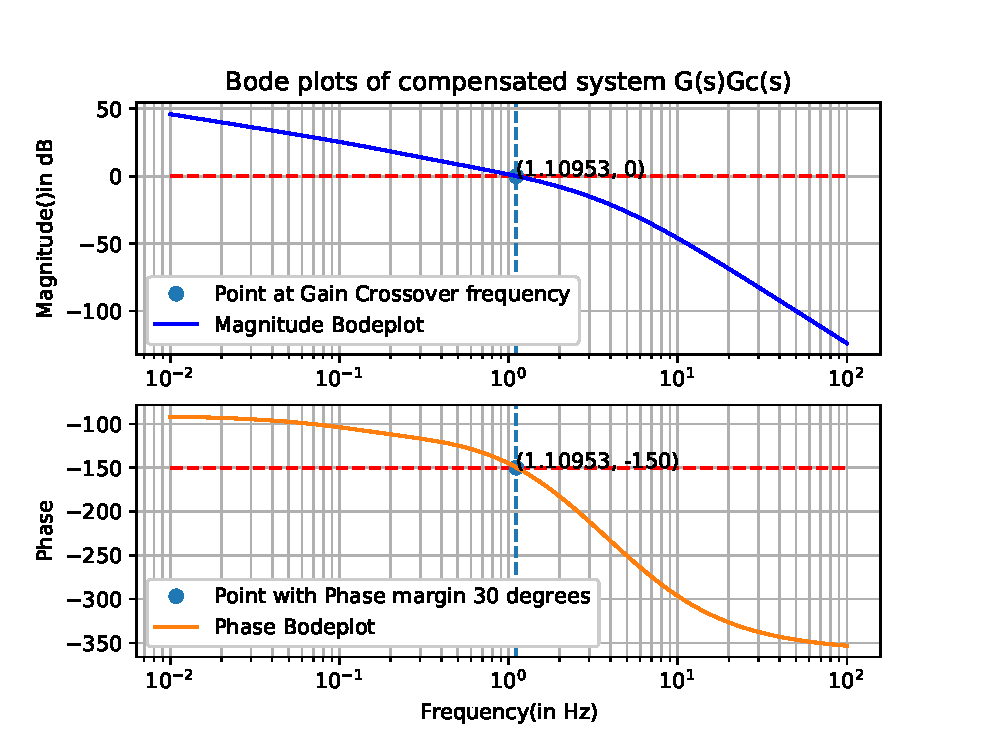
\includegraphics[width=\columnwidth]{./figs/ee18btech11046_2.eps}
\caption{}
\label{fig:ee18btech11046_compensated} 
\end{figure}
%

The code for Bode plots of compensated system 
\begin{lstlisting}
codes/ee18btech11046_2.py
\end{lstlisting}
% 

%\end{enumerate}
